\chapter{Arquitectura de SPOTPY}
Una clase setup implementa cuatro puntos de integración:
\begin{description}
\item[\texttt{parameters()}] declara priors, límites y nombres y entrega candidatos al algoritmo.
\item[\texttt{simulation(vector)}] aplica el vector al modelo y devuelve la serie simulada.
\item[\texttt{evaluation()}] entrega observaciones alineadas en longitud y orden.
\item[\texttt{objectivefunction(simulation,evaluation)}] reduce la comparación a un escalar o vector de objetivos.
\end{description}

El sampler llama repetidamente ese contrato y su base de datos añade prefijos \texttt{like*}, \texttt{par*}, \texttt{simulation\_*} y \texttt{chain}. El mejor candidato se determina respetando la orientación real: máximo para scores como NSE en DDS; mínimo para la pérdida interna de SCE-UA.

\begin{figure}[htbp]\centering
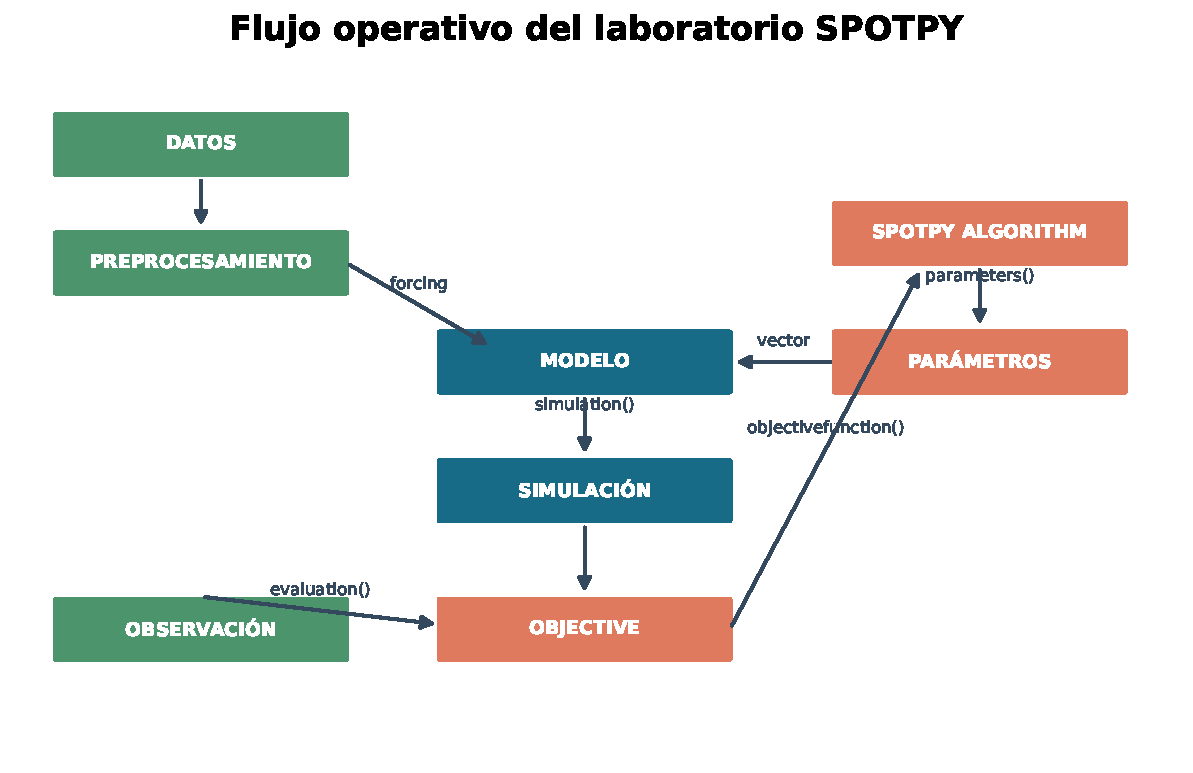
\includegraphics[width=\textwidth]{figures/spotpy_workflow.pdf}
\caption{Flujo ejecutado por el setup y el sampler.}\label{fig:workflow}
\end{figure}

La figura~\ref{fig:workflow} separa el preprocesamiento de SPOTPY. La flecha de retorno representa la decisión del algoritmo sobre el siguiente conjunto.
